%==============================================================================
%  Figure: Von Neumann Entropy S(rho) of the Market State
%  during the 2023 Banking Crisis (January–June 2023)
%
%  Placeholder TikZ/PGFPlots figure for the manuscript.
%  Compile with: pdflatex --shell-escape
%==============================================================================
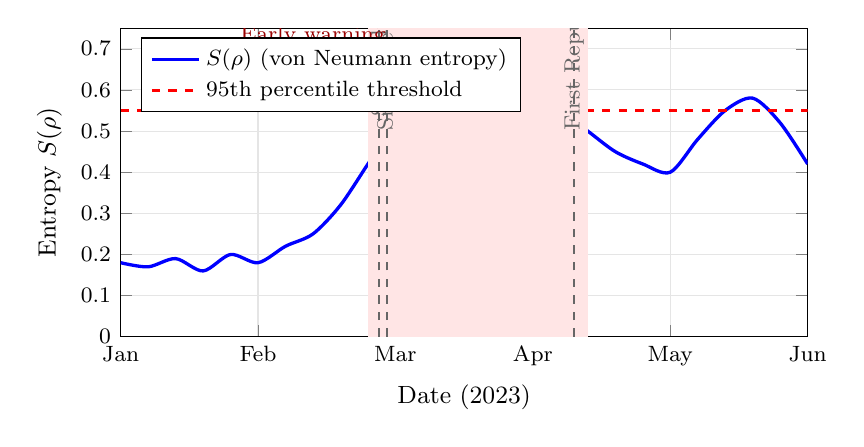
\begin{tikzpicture}
\begin{axis}[
    width=0.85\linewidth,
    height=5.5cm,
    xlabel={Date (2023)},
    ylabel={Entropy $S(\rho)$},
    xmin={2023.0}, xmax={2023.5},
    ymin={0}, ymax={0.75},
    xtick={2023.0,2023.1,2023.2,2023.3,2023.4,2023.5},
    xticklabels={Jan,Feb,Mar,Apr,May,Jun},
    ytick={0,0.1,0.2,0.3,0.4,0.5,0.6,0.7},
    legend pos=north west,
    legend cell align={left},
    grid=both,
    grid style={gray!20},
    ticklabel style={font=\footnotesize},
    label style={font=\small},
    legend style={font=\footnotesize},
]

% Von Neumann entropy S(rho) — solid blue line
% Sharp increase beginning mid-February, ~3 weeks before SVB failure
\addplot[color=blue, line width=1.2pt, smooth] coordinates {
    (2023.00, 0.18) (2023.02, 0.17) (2023.04, 0.19) (2023.06, 0.16)
    (2023.08, 0.20) (2023.10, 0.18) (2023.12, 0.22) (2023.14, 0.25)
    (2023.16, 0.32) (2023.18, 0.42) (2023.20, 0.52) (2023.22, 0.58)
    (2023.24, 0.62) (2023.26, 0.65) (2023.28, 0.63) (2023.30, 0.60)
    (2023.32, 0.55) (2023.34, 0.50) (2023.36, 0.45) (2023.38, 0.42)
    (2023.40, 0.40) (2023.42, 0.48) (2023.44, 0.55) (2023.46, 0.58)
    (2023.48, 0.52) (2023.50, 0.42)
};
\addlegendentry{$S(\rho)$ (von Neumann entropy)}

% 95th percentile threshold — horizontal dashed line
\addplot[color=red, line width=1.0pt, dashed] coordinates {
    (2023.0, 0.55) (2023.5, 0.55)
};
\addlegendentry{95th percentile threshold}

% Shaded region where S(rho) exceeds threshold
\draw[fill=red!10, draw=none] (axis cs:2023.18,0) rectangle (axis cs:2023.34,0.75);

% Vertical dashed lines for failure events
\draw[dashed, color=black!60, line width=0.8pt] (axis cs:2023.188,0) -- (axis cs:2023.188,0.75);
\node[color=black!60, font=\footnotesize, rotate=90] at (axis cs:2023.188,0.68) {SVB failure};

\draw[dashed, color=black!60, line width=0.8pt] (axis cs:2023.194,0) -- (axis cs:2023.194,0.75);
\node[color=black!60, font=\footnotesize, rotate=90] at (axis cs:2023.194,0.62) {Signature};

\draw[dashed, color=black!60, line width=0.8pt] (axis cs:2023.330,0) -- (axis cs:2023.330,0.75);
\node[color=black!60, font=\footnotesize, rotate=90] at (axis cs:2023.330,0.68) {First Republic};

% Annotation: early warning signal
\node[color=red!60!black, font=\footnotesize, align=center] at (axis cs:2023.14,0.70)
{Early warning\\signal};

\end{axis}
\end{tikzpicture}
